%\documentclass[tikz,convert={density=600,outext=.png}]{standalone}
\documentclass[tikz]{standalone}

\usepackage[utf8]{inputenc} % utf8 encoding
\usepackage[T2A]{fontenc} % use T1 fonts
\usepackage[english, russian]{babel}

%\usepackage{fontspec}
%\usepackage{polyglossia}
%\setdefaultlanguage{russian}
%\newcommand{\docfont}{Times New Roman}
%\setmainfont[Ligatures=TeX]{\docfont}
%\newfontfamily\cyrillicfont[Ligatures=TeX]{\docfont}
%\newfontfamily\cyrillicfontsf[Ligatures=TeX]{\docfont}
%\newfontfamily\cyrillicfonttt[Ligatures=TeX]{\docfont}


\usepackage{amsmath} % nice math symbols
\usepackage{tikz}
\usetikzlibrary{shapes,positioning,calc,arrows}

\newcommand{\sign}[3]{
	\filldraw[fill=white] ($(0.0,0.2)+(#2,#3)$) -- ($(0.5,1.0)+(#2,#3)$) -- ($(1.0,0.2)+(#2,#3)$) -- cycle;
	\filldraw[fill=black!20] ($(0.0,0.2)+(#2,#3)$) -- ($(0.7,0.0)+(#2,#3)$) -- ($(1.0,0.2)+(#2,#3)$) -- cycle;
	
	\draw[coord_cine] ($(0.5,1.0)+(#2,#3)$) -- ($(0.5,0.13)+(#2,#3)$);
	\draw[coord_cine] ($(0.0,0.2)+(#2,#3)$) -- ($(0.5,0.13)+(#2,#3)$);
	\draw[coord_cine] ($(0.7,0.0)+(#2,#3)$) -- ($(0.5,0.13)+(#2,#3)$);
	\draw[coord_cine] ($(1.0,0.2)+(#2,#3)$) -- ($(0.5,0.13)+(#2,#3)$);
	
	\filldraw[fill=white,fill opacity=0.8] ($(0.0,0.2)+(#2,#3)$) -- ($(0.5,1.0)+(#2,#3)$) -- ($(0.7,0.0)+(#2,#3)$) -- cycle;
	\filldraw[fill=white,fill opacity=0.8] ($(0.7,0.0)+(#2,#3)$) -- ($(0.5,1.0)+(#2,#3)$) -- ($(1.0,0.2)+(#2,#3)$) -- cycle;
	
	\node[sign_comp, fill=red] (s#1_p) at ($(0.0,0.2)+(#2,#3)$) {};
	\node[sign_comp, fill=blue] (s#1_m) at ($(1.0,0.2)+(#2,#3)$) {};
	\node[sign_comp, fill=gray] (s#1_n) at ($(0.5,1.0)+(#2,#3)$) {};
	\node[sign_comp, fill=green!70!black] (s#1_a) at ($(0.7,0.0)+(#2,#3)$) {};
	

}
% TikZ styles for drawing

\begin{document}
	
	\begin{tikzpicture}[join=round,node distance = -0.05]
		\tikzstyle{sign_comp}=[draw, circle,scale=0.7];
		\tikzstyle{coord_cine}=[dash pattern=on 0.7 off 0.7];
		
		\node {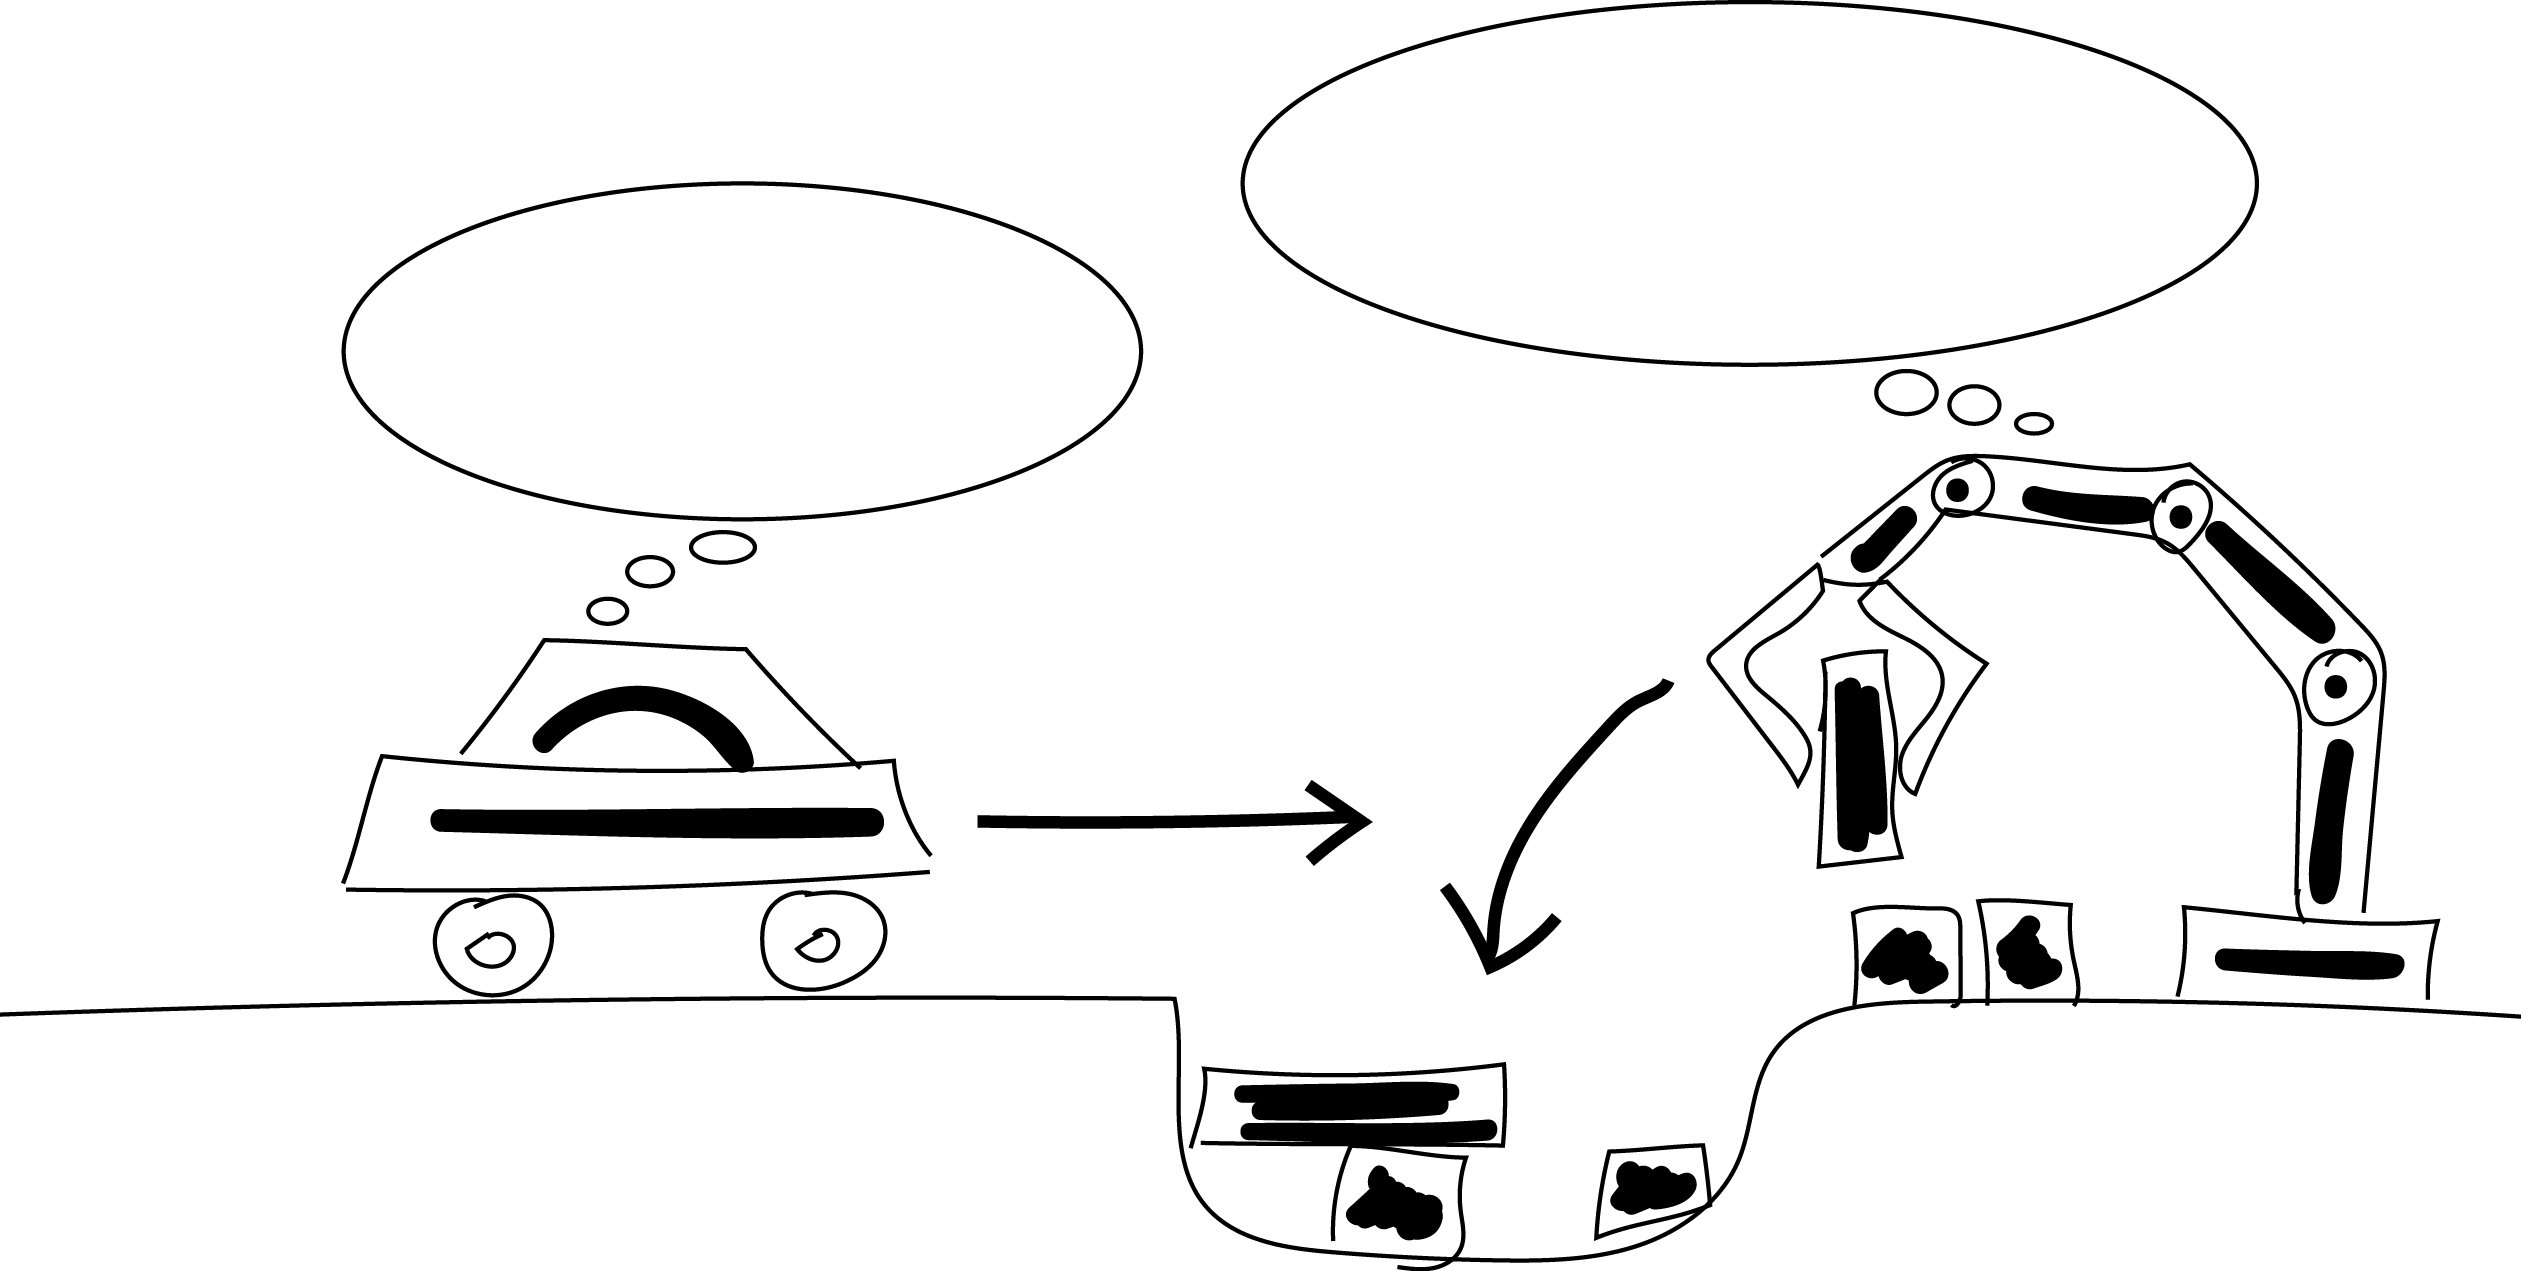
\includegraphics[width=500pt]{robo_signs.png}};
		
		
		\sign{1}{-5.8}{1.4}
		\sign{2}{-4}{1.9}
		\sign{3}{-2.5}{1.5}

		\sign{4}{1}{2.4}
		\sign{5}{2.5}{3.2}
		\sign{6}{4.1}{2.3}

		\draw[->,thick, color = blue] (s3_m) edge [bend left, out = 100, in = 90] (s2_m);
		\draw[->,thick, color = green!70!black] (s2_a) edge [bend left, out = 80, in = 120] (s1_a);
		\draw[->,thick, color = red] (s6_p) edge [bend left, out = 80, in = 120] (s5_p);
		\draw[->,thick, color = blue] (s5_m) edge [bend left, out = 80, in = 120] (s4_m);
		
		\node[draw,ellipse ,fill=gray,opacity=0.2, minimum width=40pt, minimum height = 50pt] at (-2,1.9) {};
		\node[draw,ellipse ,fill=gray,opacity=0.2, minimum width=40pt, minimum height = 50pt] at (1.5,2.8) {};
		
		\node[fill=white,fill opacity=0.9,text=black] at (-2,3) {\small препятствие};
		\node[fill=white,fill opacity=0.9, text=black] at (-3.9,3.3) {\small преграда};
		\node[fill=white,fill opacity=0.9, text=black] at (-6,2.8) {\small остановиться};
		
		\node[fill=white,fill opacity=0.9, text=black] at (1,3.9) {\small препятствие};
		\node[fill=white,fill opacity=0.9, text=black] at (4.1,4.1) {\small заполнить};
		\node[fill=white,fill opacity=0.9, text=black] at (5.4,3.2) {\small блок};
		
		\draw[<->,very thick, color = blue] (s3_m) edge [bend left, out = -80, in = -120](s4_m);
		\node at (2,1) {коммуникация};
		
		\node[align=center] at (0.4,-0.2) {Задача совместного\\преодоления\\препятствия};
	\end{tikzpicture}
\end{document}